% ----------------------------------------------------------
% Modelagem do Projeto
% ----------------------------------------------------------
\chapter{Modelagem do Projeto} \label{cha:modelagem}

% \section{Definição do produto} \label{sec:ctb:definicao}

% O projeto Calltraderbot é um bot que tem como objetivo automatizar  operações de compra e venda de criptomoedas com base em instruções dadas por usuários autorizados, nas contas de usuários clientes de exchanges integradas no referido bot. O mesmo monitora livro de ordens, preço, volume de transações de paridades com ordens criadas e se encarrega de disparar ordens com base 

% Dividido em dois grupos de usuários: Administradores e clientes. Os administradores possuem permissão para criação de instruções, que chamo de \textbf{call}, aonde informa em quais exchanges criar a ordem, o preço de entrada, o preço do alvo e uma porcentagem de perca, para um risco calculado. Os administradores também podem forçar a venda de uma call, ativar e desativar usuários clientes que acompanham seus sinais ou calls, visualizar e exportar relatórios, alterar valores de configurações, bem como todos os comandos disponíveis aos usuários clientes.

% Usuários clientes podem cadastrar chaves de acesso que permite ao bot efetuar operações de compra e venda nas exchanges, realizar um gerenciamento de risco definindo valores como percentual máximo de seu saldo a ser utilizado pelo bot e quantidade de compra por ordem, visualizar saldo, histórico de ordens, ativar e desativar negociações, bem como é notificado automaticamente pelo bot em cada alteração de status de cada ordem.

% Devido ao grande volume de transações, ordens e usuários, se viu a necessidade da criação de um gestor online para visualização dos relatórios já disponibilizados pelo bot, listando calls, ordens, usuários, suas configurações e ordens recebidas, bem como todos os dados referentes a estes elementos.

\section{Levantamento de Requisitos}
\subsection{Requisitos Funcionais}
% Os usuários administradores precisam listar e editar as configurações do canal e seus sinais em andamento, habilitar e desabilitar seus clientes (os usuários seguidores), visualizar indicadores do canal e receber notificações automáticas quando os alvos dos sinais forem atingidos e/ou novos usuários se cadastrarem. Para isso chatbot necessita ter os seguintes requisitos funcionais demonstrados na tabela a seguir:
Existe apenas um tipo de usuário no sistema e é preciso que esteja autenticado para poder utilizar as funcionalidades do sistema: Visualizar saldo, notificações, histórico de operações, ranking de usuários, participar de torneios e efetuar operações de compra e venda de ativos financeiros.

\begin{table}[htbp]
	\scriptsize
	\centering
	\begin{tabular}{|l|l|l|}
		\hline \textbf{Código} & \textbf{Requisito} & \textbf{Descrição} \\ 
		\hline RF1 & Autenticação & Registro e Login utilizando conta da Google \\
		\hline RF2 & Notificações & Receber alertas via sistema de Push Notifications \\
		\hline RF3 & Torneios & Permitir a participação de usuários em torneios \\
		\hline RF4 & Operações & Permitir comprar e vender ativos financeiros disponíveis \\
		\hline RF5 & Histórico e Ranking & Listar histórico de operações do usuário e ranking de usuários cadastrados \\
		\hline 
	\end{tabular}
	\caption{Requisitos funcionais}
	\label{tab:requisitos_funcionais_admin}
\end{table}

\subsection{Requisitos Não Funcionais}

Sobre os requisitos relacionados ao ambiente onde a aplicação está inserida, como: Um servidor mais robusto, medidas de segurança ou um usuário especializado para realização de determinadas ações. Não devem ser ignorados por não fazerem parte diretamente da aplicação, mas devem ser considerados por compor o seu ambiente e, por vezes, determinante para a sua utilização. Como os relacionados na tabela a seguir:

\begin{table}[htbp]
	\scriptsize
	\centering
	\begin{tabular}{|l|l|l|}
		\hline \textbf{Código} & \textbf{Requisito} & \textbf{Descrição} \\ 
		\hline RNF1 & O sistema deve ser simples e intuitivo, provendo rapidez e facilidade nas interações & Usabilidade \\
		\hline RNF2 & A Aplicação deve garantir a identificação do usuário & Segurança \\
		\hline RNF3 & A Aplicação deve realizar as operações de compra e venda em menos de 5 segundos & Desempenho \\
		\hline RNF4 & A Aplicação deve ser compatível com Android 6.0 ou superior & Compatibilidade \\
		\hline 
	\end{tabular}
	\caption{Requisitos não-funcionais}
	\label{tab:requisitos_funcionais_admin}
\end{table}

\section{Diagramas de casos de uso} \label{sec:modelagem:casos}

O diagrama de caso de uso desenvolvido mostrado na figura \ref{fig:uml_caso_uso} descreve as possíveis interações do usuário através da ferramenta.

\begin{figure}[H]
  \caption{\label{fig:uml_caso_uso}Diagrama UML de Casos de Uso}
  \centering
  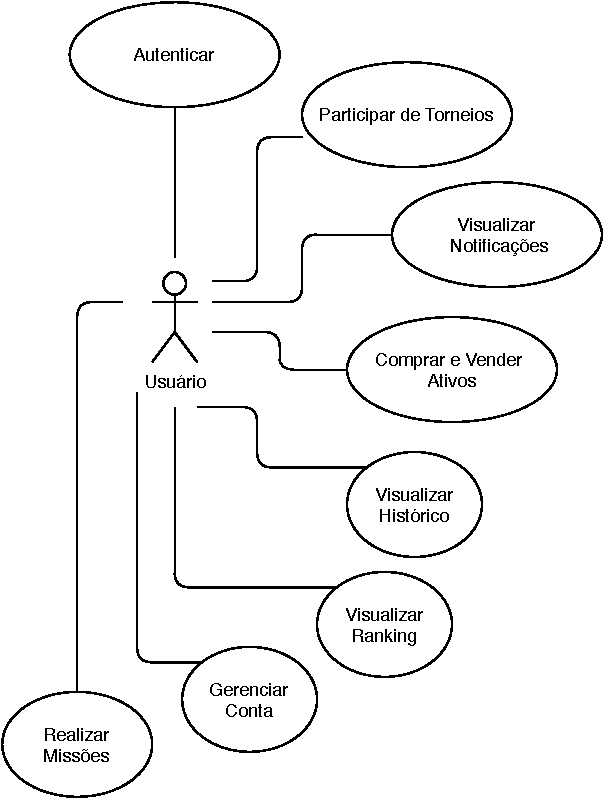
\includegraphics[scale=1]{imagens/tfc_use_case.pdf}
  \legend{Fonte: Elaborado pelo Autor}
\end{figure}

A partir deste diagrama foi criado os seguintes casos de uso:

\begin{lista}
  \item \textbf{Caso de Uso 01 - Autenticar}: O usuário utilizando sua conta Google autentica-se no sistema;
  \item \textbf{Caso de Uso 02 - Participar de torneios}: O usuário pode competir com outros usuários através de torneios periódicos disponíveis na plataforma;
  \item \textbf{Caso de Uso 03 - Visualizar notificações}: Através da gaveta de notificações o usuário pode visualizar os alertas recebidos;
  \item \textbf{Caso de Uso 04 - Comprar e vender ativos}: O usuário pode negociar ativos financeiro;
  \item \textbf{Caso de Uso 05 - Visualizar histórico}: O usuário pode visualizar o histórico de suas negociações e evolução de seu saldo;
  \item \textbf{Caso de Uso 06 - Visualizar ranking}: É disponibilizado um ranking categórico aos usuários;
  \item \textbf{Caso de Uso 07 - Gerenciar conta}: O usuário pode alterar dados referentes a sua conta;
  \item \textbf{Caso de Uso 08 - Realizar missões}: O usuário visualiza as missões diárias disponíveis a fim de ganhar recompensas;
\end{lista}

Os documentos com as especificações completas estão disponíveis no Anexo \ref{anexo:a} deste trabalho.

\section{Diagramas de classe} \label{sec:modelagem:classe}

O modelo de dados da aplicação apresentado na Figura \ref{fig:uml_der}, onde é apresentado um diagrama UML de classes do projeto model. Estas são as principais entidades do sistema e seus relacionamentos:

\begin{lista}
  \item \textbf{User}: Representa um usuário cadastrado do sistema;
  \item \textbf{Asset}: Representa um ativo financeiro;
  \item \textbf{Belt}: Representa uma categorização do usuário, de acordo com sua performance da negociação de ativos;
  \item \textbf{Tournament}: Representa uma competição entre usuários em um determinado período de tempo;
  \item \textbf{Mission}: Representa um desafio com recompensa a fim de engajar o usuário;
\end{lista}

\section{Arquitetura do Sistema} \label{sec:modelagem:arquitetura}
\section{Diagrama de Entidades-Relacionamentos} \label{sec:modelagem:der}

Na figura \ref{fig:uml_der} podemos ver a estrutura lógica usada como base para o banco de dados.

\begin{figure}[H]
  \caption{\label{fig:uml_der}Diagrama entidade-relacionamento}
  \centering
  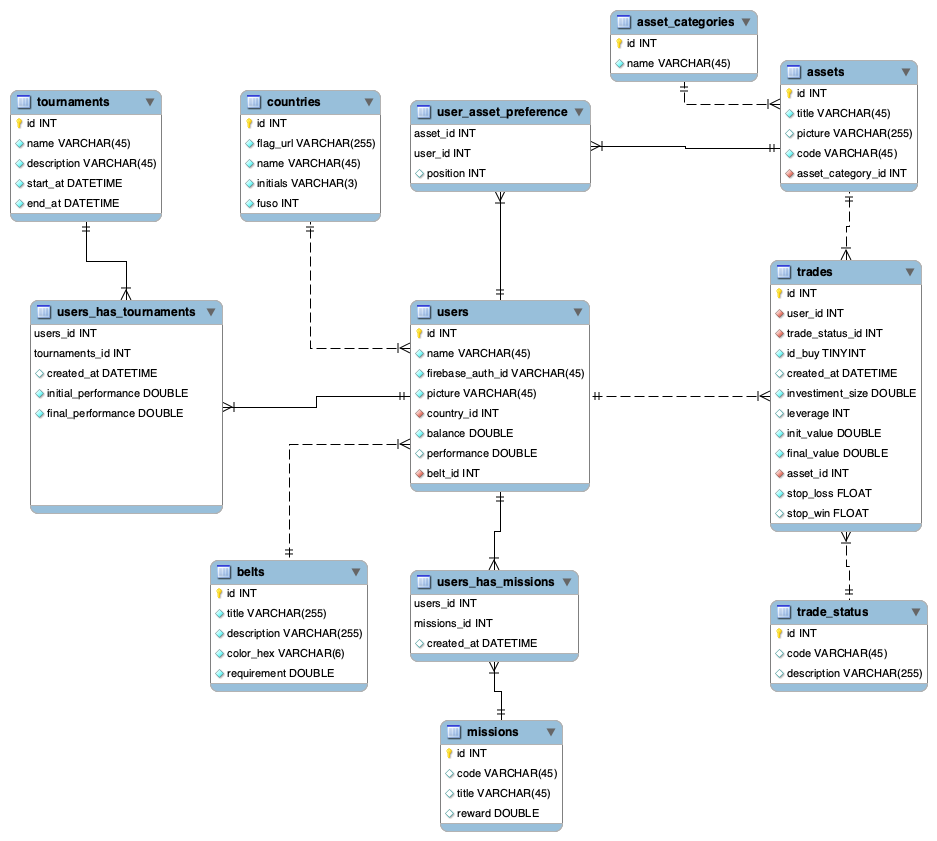
\includegraphics[scale=0.5]{imagens/tfc_der.png}
  \legend{Fonte: Elaborado pelo Autor}
\end{figure}

\section{Interface} \label{sec:modelagem:interface}